\section{Results and Analysis}
\label{sec:results}

\subsection{Same-Cache Projection Ablation}

Table~\ref{tab:ablation} is the primary causal comparison. Relative to
\textsc{REL-U}, IHP raises equal-subdataset F1-max from 0.6354 to 0.6621,
AUPRC from 0.2974 to 0.3192, and VUS-PR from 0.6873 to 0.6975. The observed
differences are +0.0267, +0.0218, and +0.0102. The unadjusted intervals
exclude zero for AUPRC and VUS-PR, while the F1-max interval extends to
-0.0023. These intervals describe sampling variability under the paired
benchmark hierarchy and are not adjusted for the component-arm selection
disclosed in Section~\ref{sec:experiments}.

\begin{table}[t]
  \centering
  \caption{Same-cache projection ablation on 492 paired series. Intervals use
  10,000 hierarchical bootstrap replicates and are unadjusted for arm
  selection. ``Positive'' counts subdatasets with a positive IHP-minus-
  \textsc{REL-U} difference.}
  \label{tab:ablation}
  \footnotesize
  \resizebox{\columnwidth}{!}{%
  \begin{tabular}{lrrrrr}
    \toprule
    Metric & \textsc{REL-U} & IHP & $\Delta$ & 95\% interval & Positive \\
    \midrule
    F1-max & .6354 & .6621 & +.0267 & [-.0023, .0681] & 6/11 \\
    AUPRC  & .2974 & .3192 & +.0218 & [.0062, .0398] & 9/11 \\
    VUS-PR & .6873 & .6975 & +.0102 & [.0021, .0197] & 7/11 \\
    \bottomrule
  \end{tabular}%
  }
\end{table}

The subdataset distribution shows that the ranking gains are not confined to
one family. IHP improves AUPRC on 9/11 groups, with its largest gains on
Yahoo-A1 (+0.0768) and Yahoo-A2 (+0.0584); the largest AUPRC loss is -0.0116
on NAB-Tweets. VUS-PR gains most on Yahoo-A1 (+0.0367) and Yahoo-A2
(+0.0360), whereas its largest loss is -0.0053 on NASA-SMAP. F1-max is more
heterogeneous: IHP gains +0.1680 on NAB-Artificial and +0.0913 on NAB-Traffic
but loses -0.0174 on NASA-SMAP. This heterogeneity is consistent with the
wider F1-max interval and its arm-specific maximizing operating point.

\begin{figure*}[t]
  \centering
  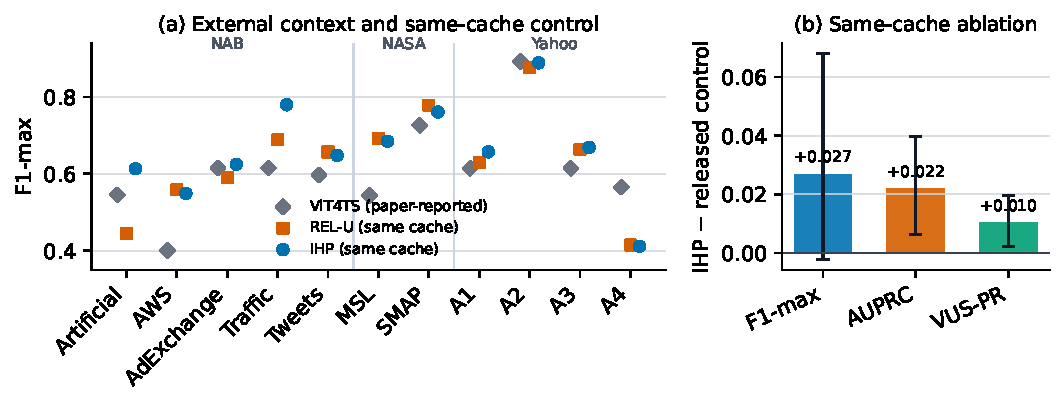
\includegraphics[width=0.97\textwidth]{figures/ihp_results.pdf}
  \caption{Full evidence summary. (a) External paper-reported ViT4TS and the
  two local same-cache F1-max arms across eleven categorical subdatasets; the
  markers are intentionally unconnected. (b) Same-cache IHP-minus-
  \textsc{REL-U} differences with unadjusted hierarchical 95\% intervals.
  The F1-max interval crosses zero; the AUPRC and VUS-PR intervals do not.}
  \label{fig:results}
\end{figure*}

\subsection{External Paper-Reported Context}

Table~\ref{tab:external} separates the paper-reported ViT4TS values from the
two local same-cache arms. IHP obtains equal-subdataset F1-max 0.662 versus
the external ViT4TS value 0.612 and is numerically higher on 9/11
subdatasets. However, the local released-coordinate control already obtains
0.635; consequently, the external +0.050 difference is not the IHP effect.
The attributable local difference is the paired +0.027 reported above.

\begin{table}[t]
  \centering
  \caption{Complete F1-max context for the VLM4TS Table~1 taxonomy.
  ViT4TS$^{\mathrm{P}}$ is external and paper-reported; \textsc{REL-U}, IHP,
  and $\Delta_{\mathrm{pair}}$ are local same-cache results. Cross-environment
  columns are not a paired ranking.}
  \label{tab:external}
  \footnotesize
  \setlength{\tabcolsep}{2.3pt}
  \resizebox{\columnwidth}{!}{%
  \begin{tabular}{lrrrrr}
    \toprule
    Subdataset & $n$ & ViT4TS$^{\mathrm{P}}$ & \textsc{REL-U} & IHP & $\Delta_{\mathrm{pair}}$ \\
    \midrule
    NAB-Artificial & 6   & .545 & .445 & .613 & +.168 \\
    NAB-AWS        & 17  & .400 & .558 & .549 & -.009 \\
    NAB-AdExchange & 5   & .615 & .590 & .624 & +.034 \\
    NAB-Traffic    & 7   & .615 & .688 & .779 & +.091 \\
    NAB-Tweets     & 10  & .597 & .656 & .648 & -.009 \\
    NASA-MSL       & 27  & .543 & .692 & .684 & -.008 \\
    NASA-SMAP      & 53  & .726 & .778 & .760 & -.017 \\
    Yahoo-A1       & 67  & .614 & .628 & .657 & +.029 \\
    Yahoo-A2       & 100 & .892 & .876 & .888 & +.013 \\
    Yahoo-A3       & 100 & .614 & .663 & .669 & +.005 \\
    Yahoo-A4       & 100 & .565 & .415 & .411 & -.003 \\
    \midrule
    Equal-11       & 492 & .612 & .635 & .662 & +.027 \\
    \bottomrule
  \end{tabular}%
  }
\end{table}

The full paper-reported VLM4TS system reaches 0.659, but it adds an external
language-model verification stage absent from both local arms. We therefore
do not use it as a paired comparator. Yahoo-A4 further illustrates the
environment boundary: IHP is 0.154 below the external ViT4TS entry but only
0.003 below the local control, while its same-cache AUPRC and VUS-PR increase
by 0.0157 and 0.0069. This discrepancy is compatible with threshold and
environment differences and prevents a causal reading of the external rows.

\subsection{Structural Certificate and Computational Boundary}

Table~\ref{tab:certificate} tests the mechanism without labels. At both
pooled scales, every one of the 195 released queries that finds support is
shifted by one flattened cell. Thirteen of those shifts wrap across row
boundaries, and the terminal query is unsupported. Literal incidence covers
all 196 output cells. The medium and large mask hashes are identical across
all 492 cached transactions, so the certificate is not inferred from a
single selected series.

\begin{table}[t]
  \centering
  \caption{Label-free support-graph certificate on the $14\times14$ grid.
  ``Rel. valid'' counts shifted queries returning support; all 195 are
  displaced. ``Row wraps'' is the subset crossing a row boundary.}
  \label{tab:certificate}
  \footnotesize
  \resizebox{\columnwidth}{!}{%
  \begin{tabular}{lrrrrr}
    \toprule
    Scale & Output & Rel. valid & IHP valid & Row wraps & Holes \\
    \midrule
    Medium & 196 & 195 & 196 & 13 & 1 \\
    Large  & 196 & 195 & 196 & 13 & 1 \\
    \bottomrule
  \end{tabular}
  }
\end{table}

IHP introduces zero trainable parameters, consumes no labels, and reuses the
same CLIP token cache. All 492 paired manifests agree in cache key, token hash,
cache-manifest hash, and encoder-call count. Replacing \textsc{REL-U} with IHP
therefore adds zero token-cache bytes and preserves the persisted score
footprint (11.82~MiB for all 492 series). It also adds no encoder pass or
external-VLM call; only the fixed incidence lookup changes before the
inherited harmonic reduction. Runtime and peak allocated VRAM were recorded
jointly for three experimental arms, so we make no arm-isolated latency, VRAM,
or host-RAM claim. The exact certificate and paired threshold-free
improvements support the narrower conclusion that the projection interface,
rather than additional model capacity, changes the anomaly ranking.
